\documentclass[11pt,a4paper,english]{article}
\usepackage[T1]{fontenc}
\usepackage[utf8]{inputenc}
\usepackage{babel}
\usepackage{geometry}
    \geometry{
    	left=2cm,
	right=2cm,
	includeheadfoot, top=1cm, bottom=1cm,
    headsep=2cm,
    footskip=2.5cm
    }
\usepackage{fancyhdr}
\usepackage{lipsum}
\usepackage{import}

% Extensions file
\import{"/Users/aron/Google Drive/TEMPLATES/"}{falcon.tex} % path filled by fasttex in .zprofile

% Setup for page layout (fancyhdr)
\fancyhf{}
\lhead{Aron Fiechter}
\chead{UROP 2017}
\rhead{\today}
\cfoot{\thepage}
\pagestyle{fancy}

\begin{document}

    {\centering\huge\textbf{Project report}\par}

    \vspace{1cm}
    
    \section{Overview}
	
	The goal of this project was to develop an extension for the drawing application Ipe that allows to draw the Farthest Line Segment Voronoi Diagram (FSVD); such an extension is called an Ipelet.\par
	The Computational Geometry Algorithms Library (CGAL) for \cod{C++} offers a good support to develop Ipelets.\par
	This project's repository is available on \href{https://github.com/Spyridox/UROP2017-FSVD}{Github at https://github.com/Spyridox/UROP2017-FSVD}.
	
	\subsection{FSVD}
	
	The Farthest Line Segment Voronoi Diagram is a planar arrangement  constructed for a set of line segments. It has faces, edges and vertices and it represents the region (called Voronoi region) of points that are farthest from a given segment, for all segments; for some segments, this region could also be constituted by two or more separate parts; for others, this region might even	 be empty. The edges of a FSVD always form a tree, and the diagram is therefore never disconnected (unlike the Nearest Line Segment Voronoi Diagram, where the edges can be in up to \(n -1\) disconnected parts, for a diagram for \n segments).\par
	See examples below, with segments in dark and the diagrams in orange (figure \ref{fig:examples}).
	
	\begin{figure}[h]
    \centering
    \begin{subfigure}[b]{0.45\textwidth}
        \fbox{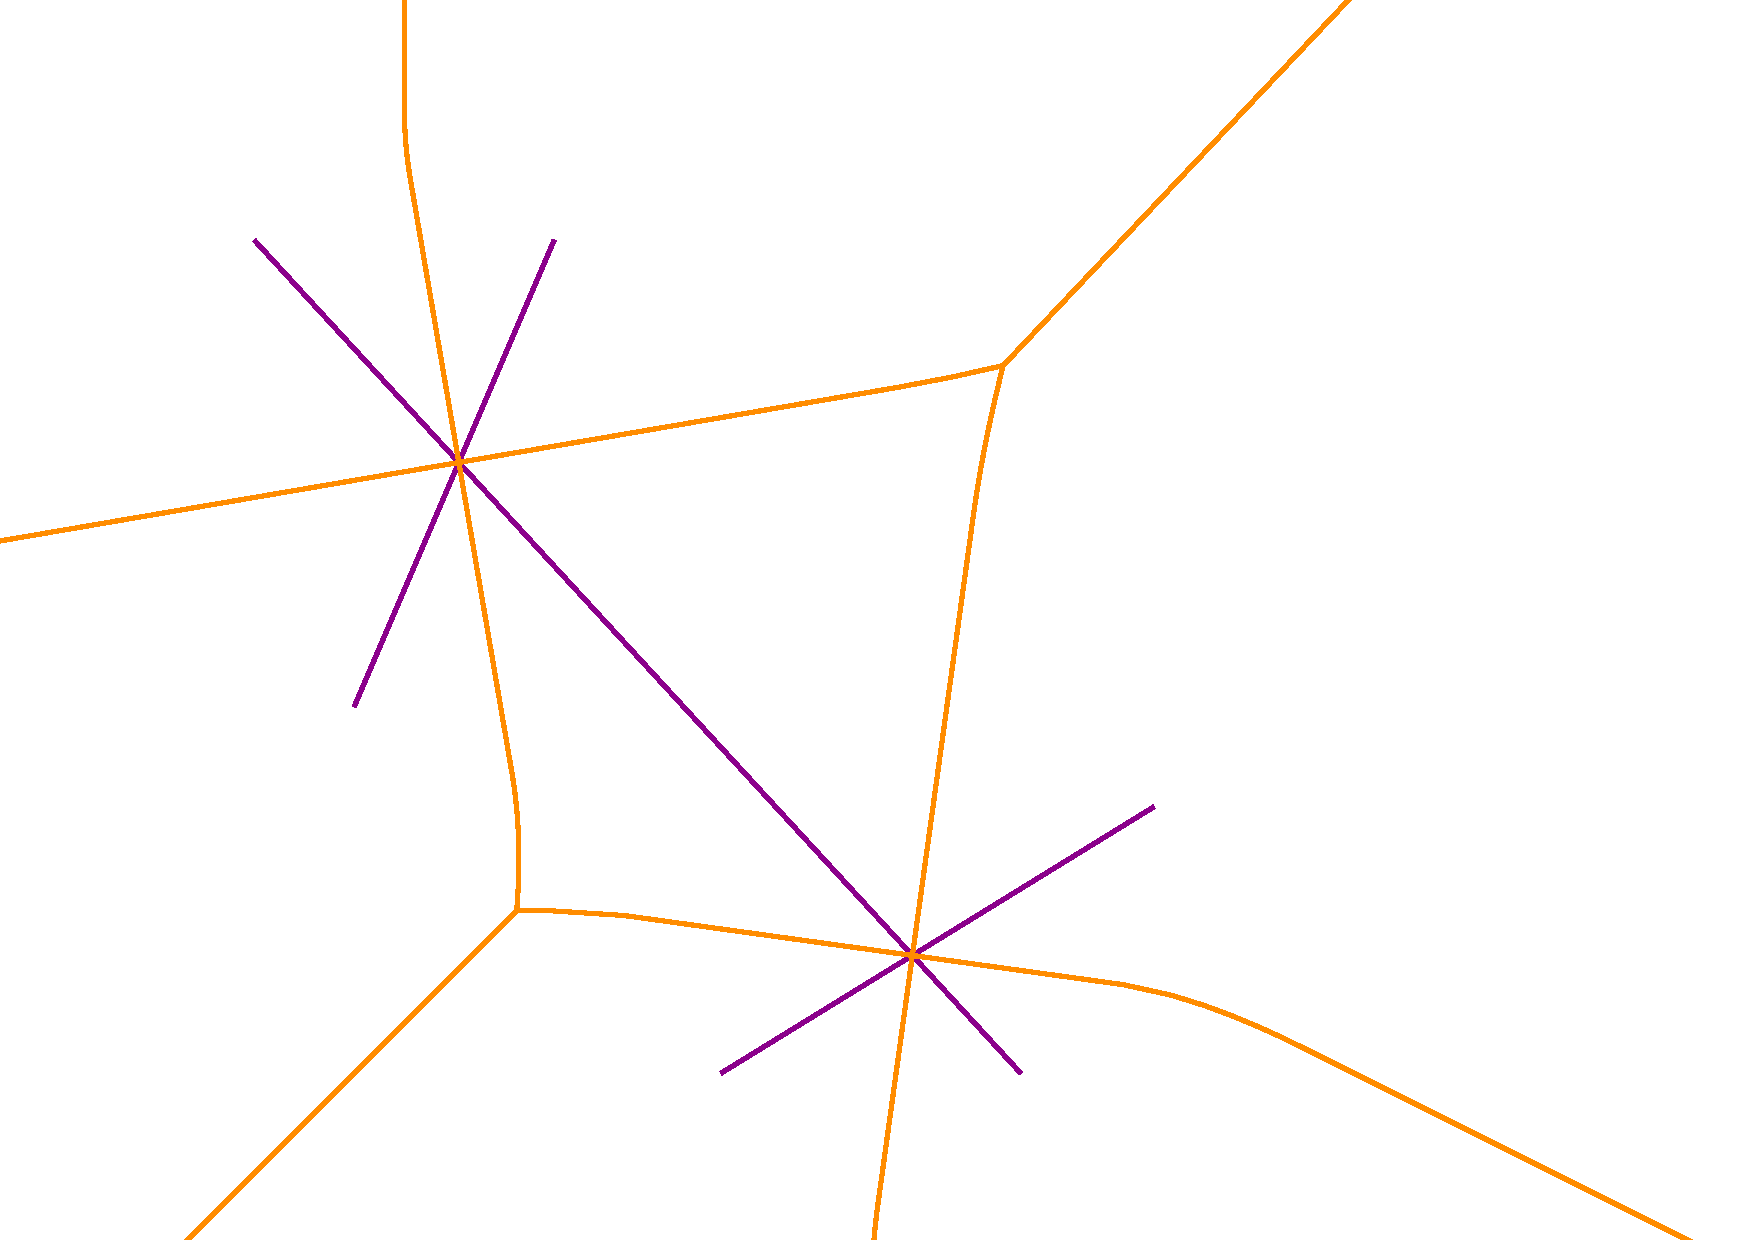
\includegraphics[width=\textwidth]{SVD_example}}
        \caption{Nearest\label{fig:SVD_example}}
    \end{subfigure}
	\qquad
    \begin{subfigure}[b]{0.45\textwidth}
        \fbox{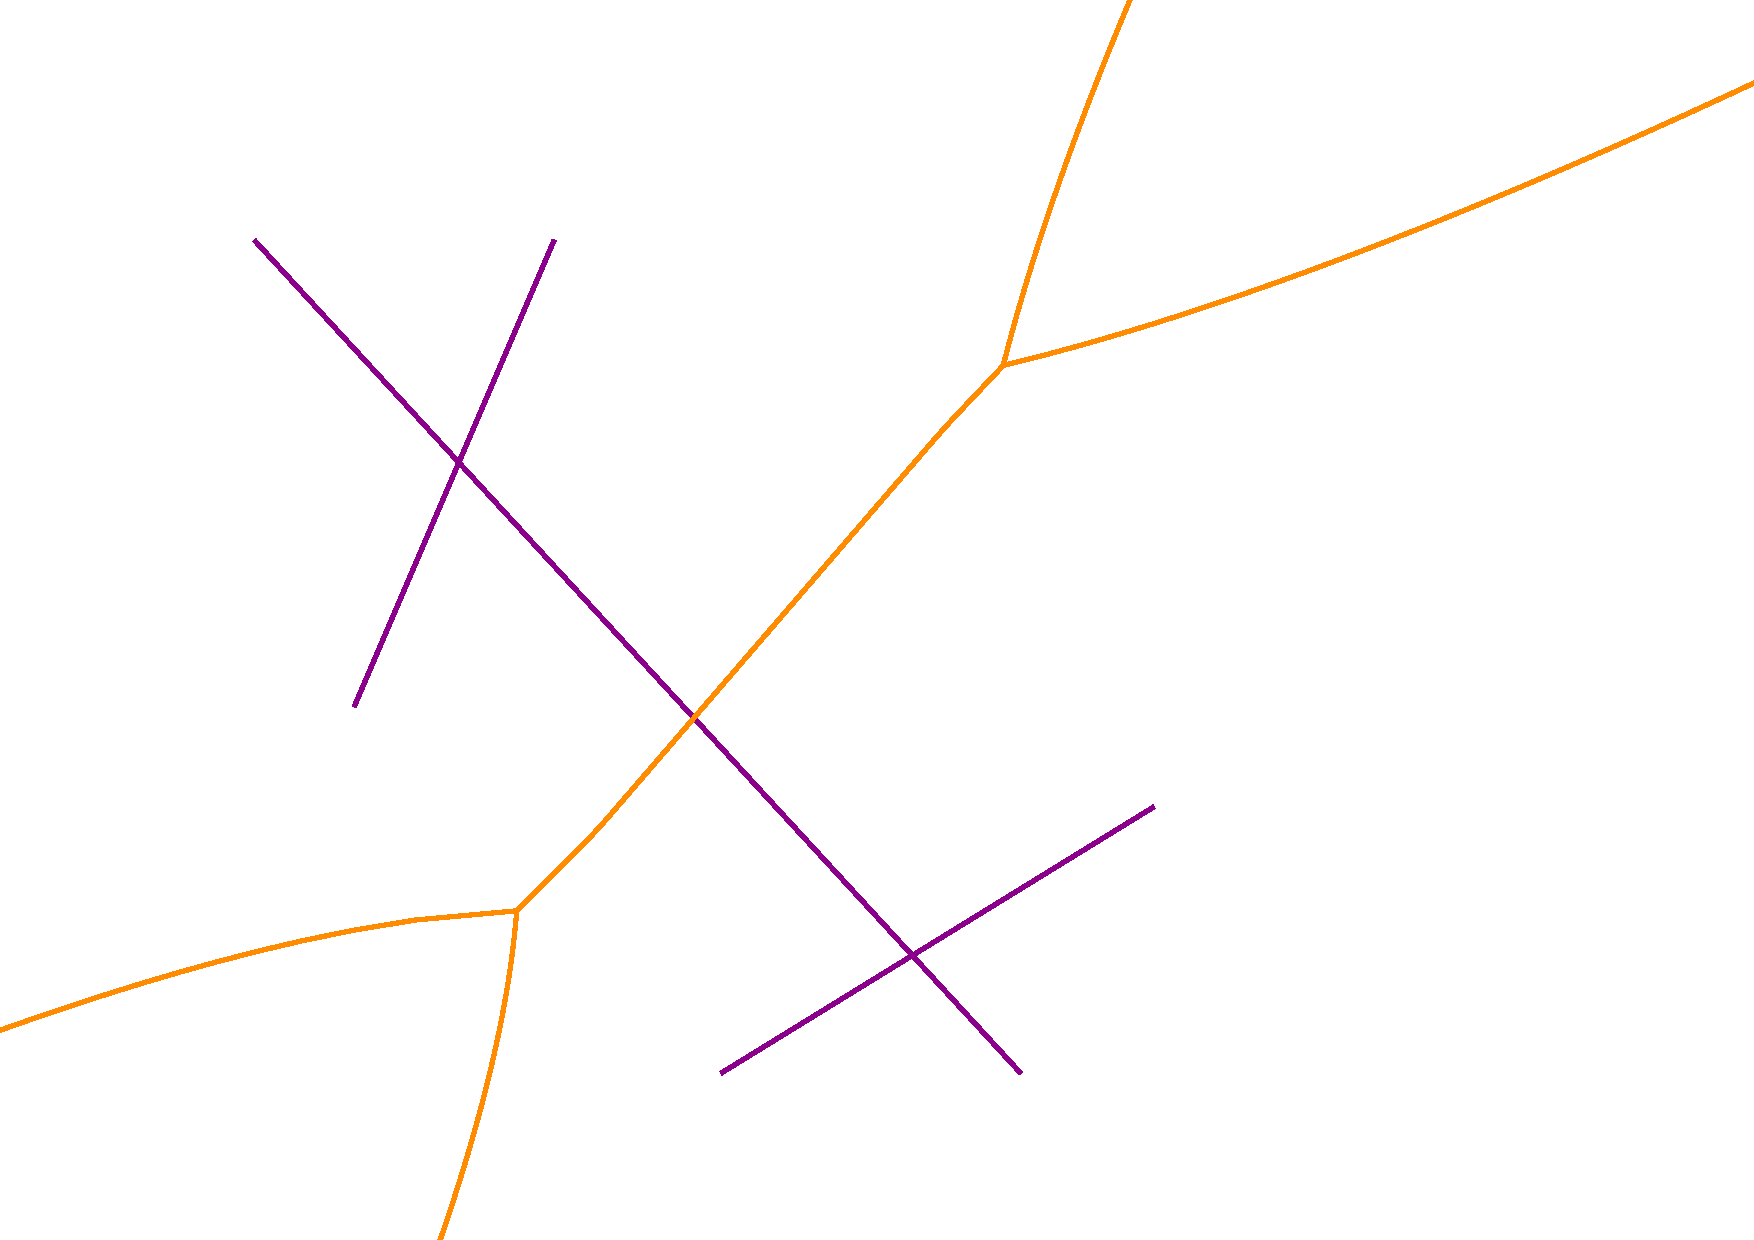
\includegraphics[width=\textwidth]{FSVD_example}}
        \caption{Farthest\label{fig:FSVD_example}}
    \end{subfigure}
    \caption{Voronoi diagrams with line segments\label{fig:examples}}
	\end{figure}
	
	For figure \ref{fig:FSVD_example}, the region of the two smaller segments are the two larger ones, each opposed to its segment. The two smaller parts are the two pieces of the region of the longest segment.
	
	\subsection{CGAL and Ipelets}
	
	In this project two new functions were added to an Ipelet that already featured functions to construct Voronoi diagrams of points, Voronoi diagrams for segments, points and polygons using the \(L_{\infty}\) metric, farthest color and Hausdorff Voronoi diagrams.\par
	The two functions added are to construct, under \(L_{2}\) metric, the nearest and the farthest Voronoi diagram for line segments.\par
	For both cases the concept used is to represent the distance function of each segment as a surface, then take either the upper or the lower envelope of these surfaces (for FSVD and SVD respectively).
	
	\subsection{The envelopes strategy}
	For a single segment on the \(xy\)-plane, for every point plot on the \(z\) axis the distance of that point to the segment. This creates an (unlimited) 3D surface. For a point, this surface is simply a cone; for a segment, it's two haflcones originating at the endpoints of the segment and two planes originating from the inner part of the segment (figure \ref{fig:distance_function}).\par
	\begin{figure}[h]
    \centering
    \framebox{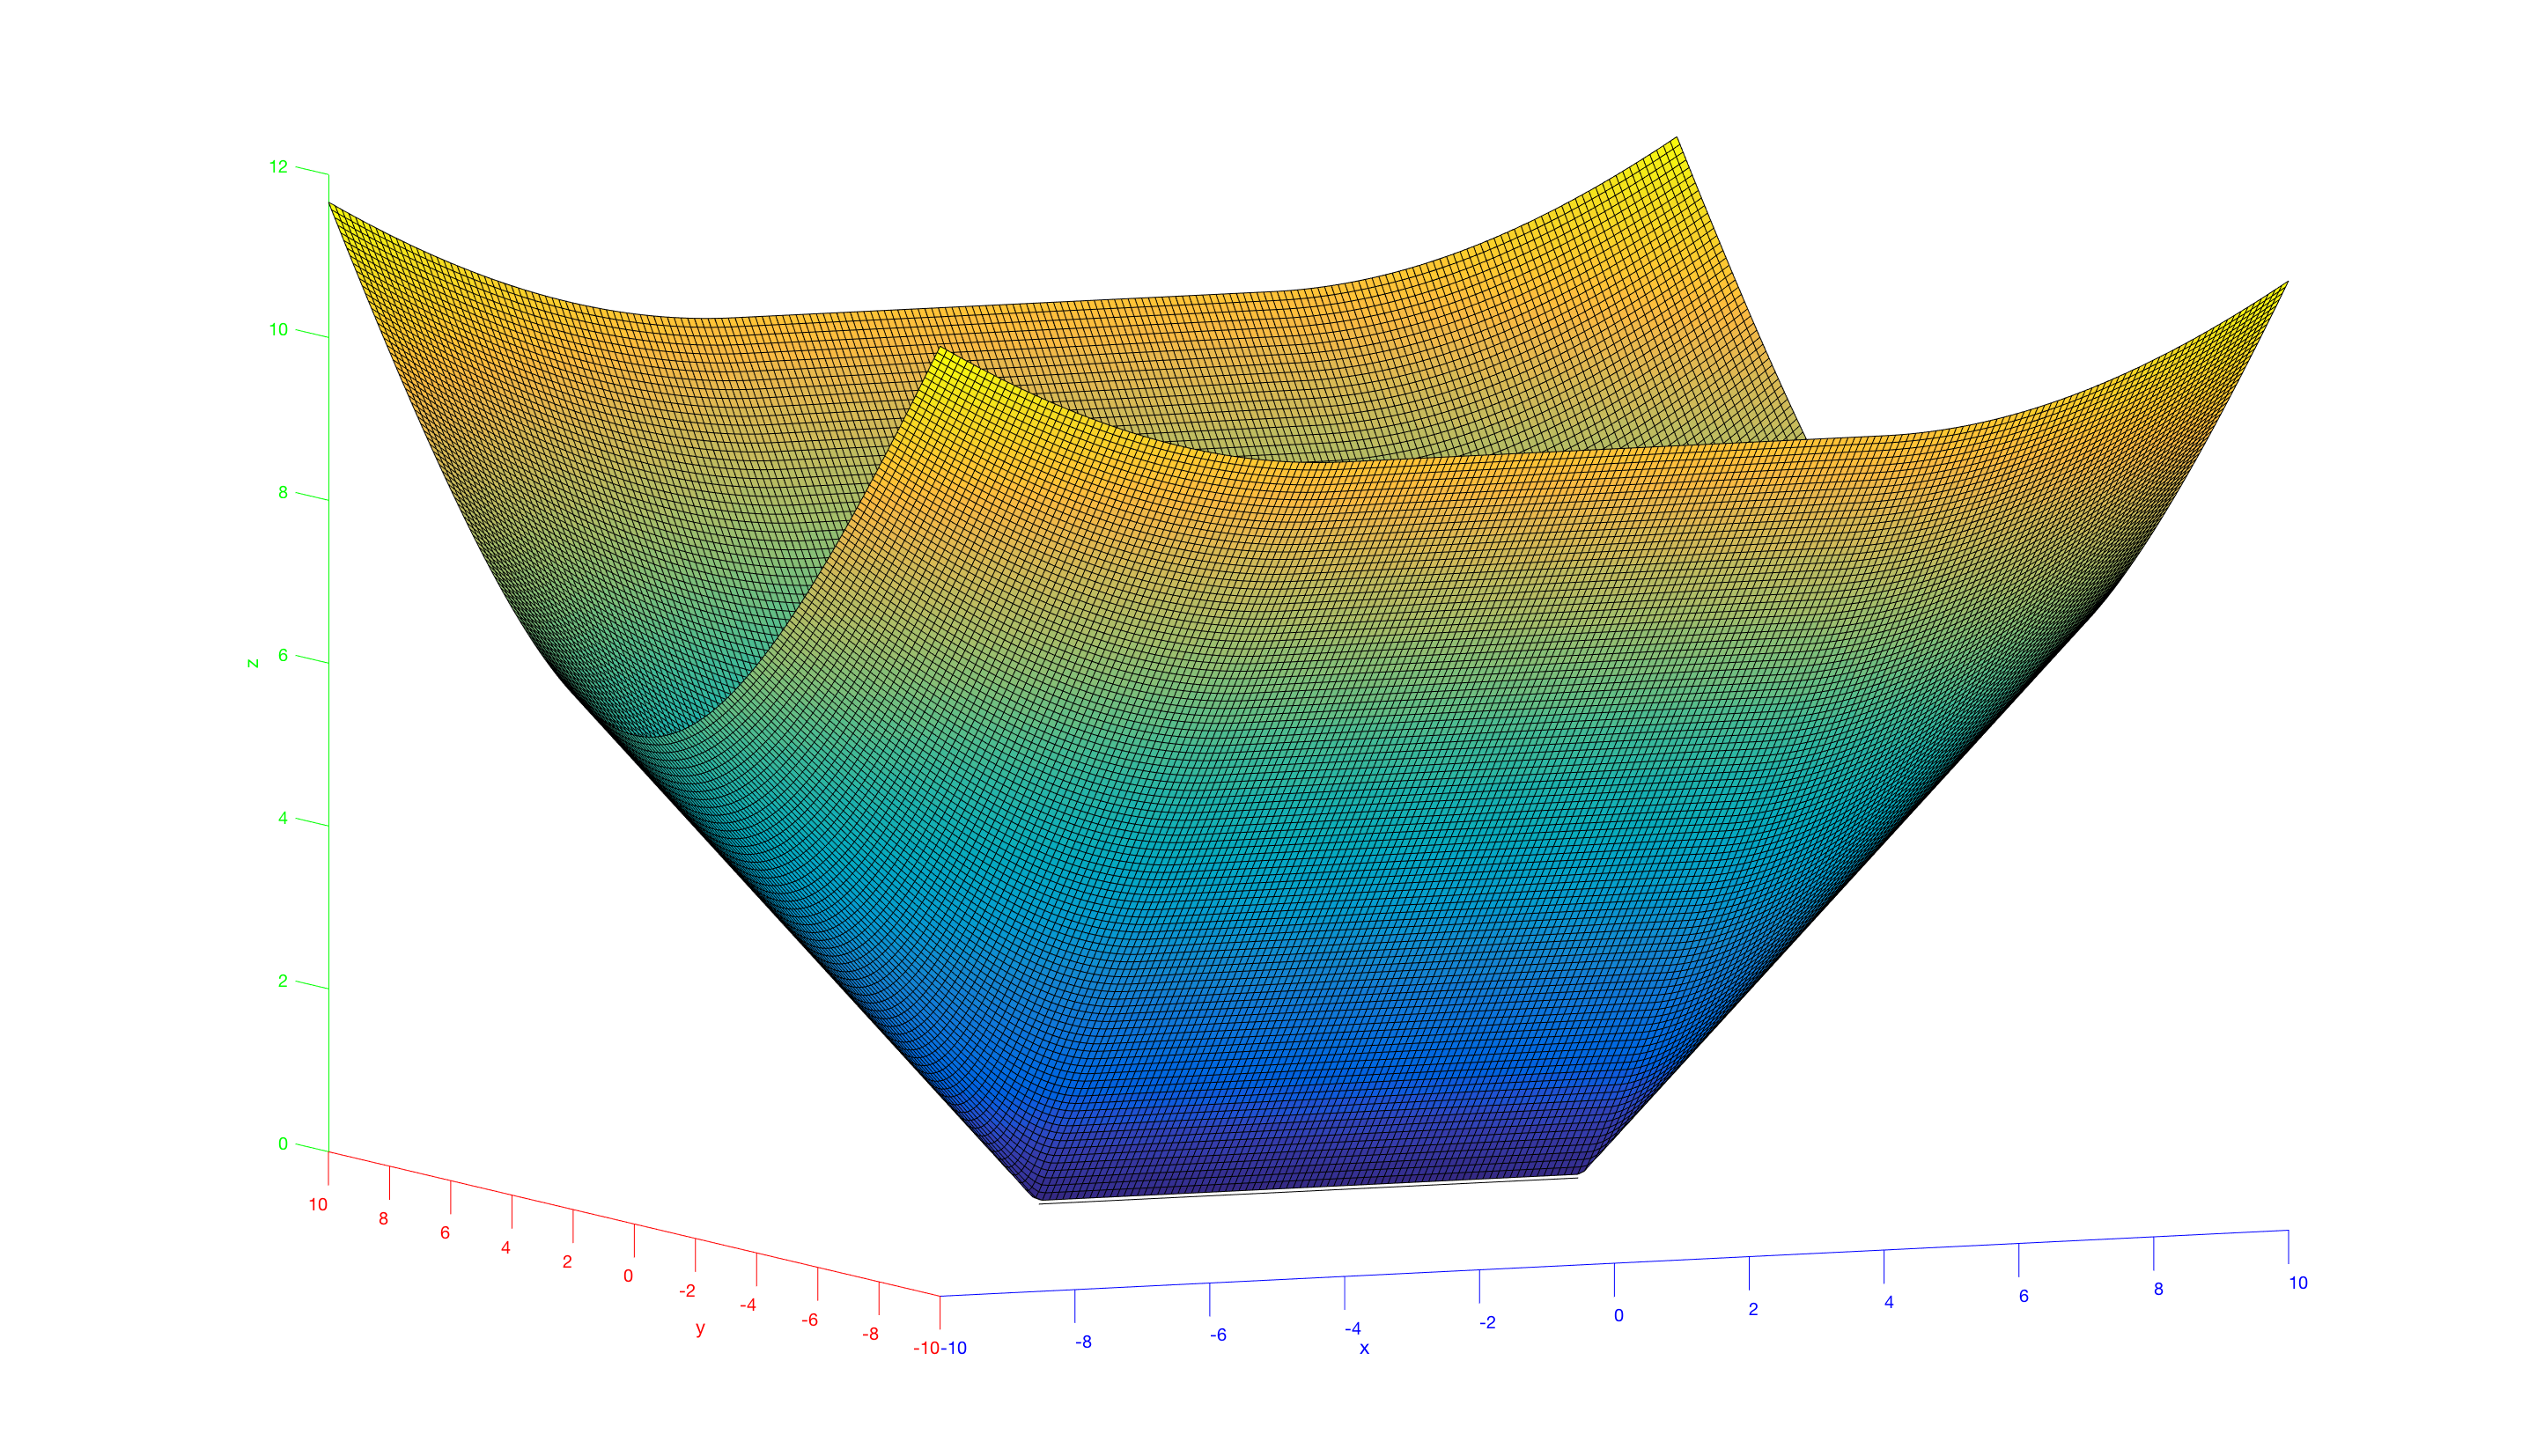
\includegraphics[width=0.8\textwidth]{distance_function}}
    \caption{Distance function surface for a segment\protect\footnotemark \label{fig:distance_function}}
	\end{figure}
	\footnotetext{created using MATLAB script by Martin Suderland}
	For two distinct segments, these distance function surfaces intersect, and their intersection projected back onto the \(xy\)-plane is simply the planar euclidean bisector of the two segments.\par
	For many segments, given all their distance function surfaces, if the lower envelope is taken then the \(xy\)-projection of this envelope is the nearest Voronoi diagram, whereas the \(xy\)-projection of the upper envelope is the farthest Voronoi diagram.
	
	%____________________________________________________________

	\section{Envelope package and \cod{Envelope_diagram_2<EnvTraits>}}
	CGAL features a package to compute envelopes and their projections. The methods \cod{upper_envelope_3} and \cod{lower_envelope_3} output the resulting \(xy\)-projection diagrams in a \cod{Envelope_diagram_2} object.\par
	This diagram class is parametrised by a traits class that must define the geometry of the surfaces that it handles; to do so, it needs to support construction of the projected boundary of a single surface, the construction of the projection of the intersection of two surfaces, as well as other functions to determine the z-order of two surfaces in specific cases (more specifically, the traits class must be a model of the concept \cod{EnvelopeTraits_3}, specified on the \href{https://doc.cgal.org/4.9.1/Envelope_3/classEnvelopeTraits__3.html}{CGAL documentation}).\par
	There are already traits classes to support construction of envelopes of spheres, triangles and planes, but these did not include what we needed for FSVD, so a new class needed to be developed.
	
	\subsection{Traits class \cod{L2_segment_voronoi_traits_2<ArrTraits_2>}}
	The \cod{EnvelopeTraits_3} concept requires any model to define the types \cod{Surface_3} and \cod{X_monotone_surface_3}, but it allows the surfaces to be any kind of object, as long as the other required functions do their task correctly. Because of this, for FSVD (and SVD too, they can use the same traits class) the surfaces are defined to be simply the segments themselves, since they contain all the information needed for the computations.\par
	In the function that requires to compute the projected intersection of two surfaces, we can in fact directly compute the planar euclidean bisector of the two segments.\par
	The bisector is formed, in the general case, by unbounded rays, segments and parabolic arcs (figure \ref{fig:areas_of_influence}).\ppar
	\begin{figure}[h]
    \centering
    \framebox{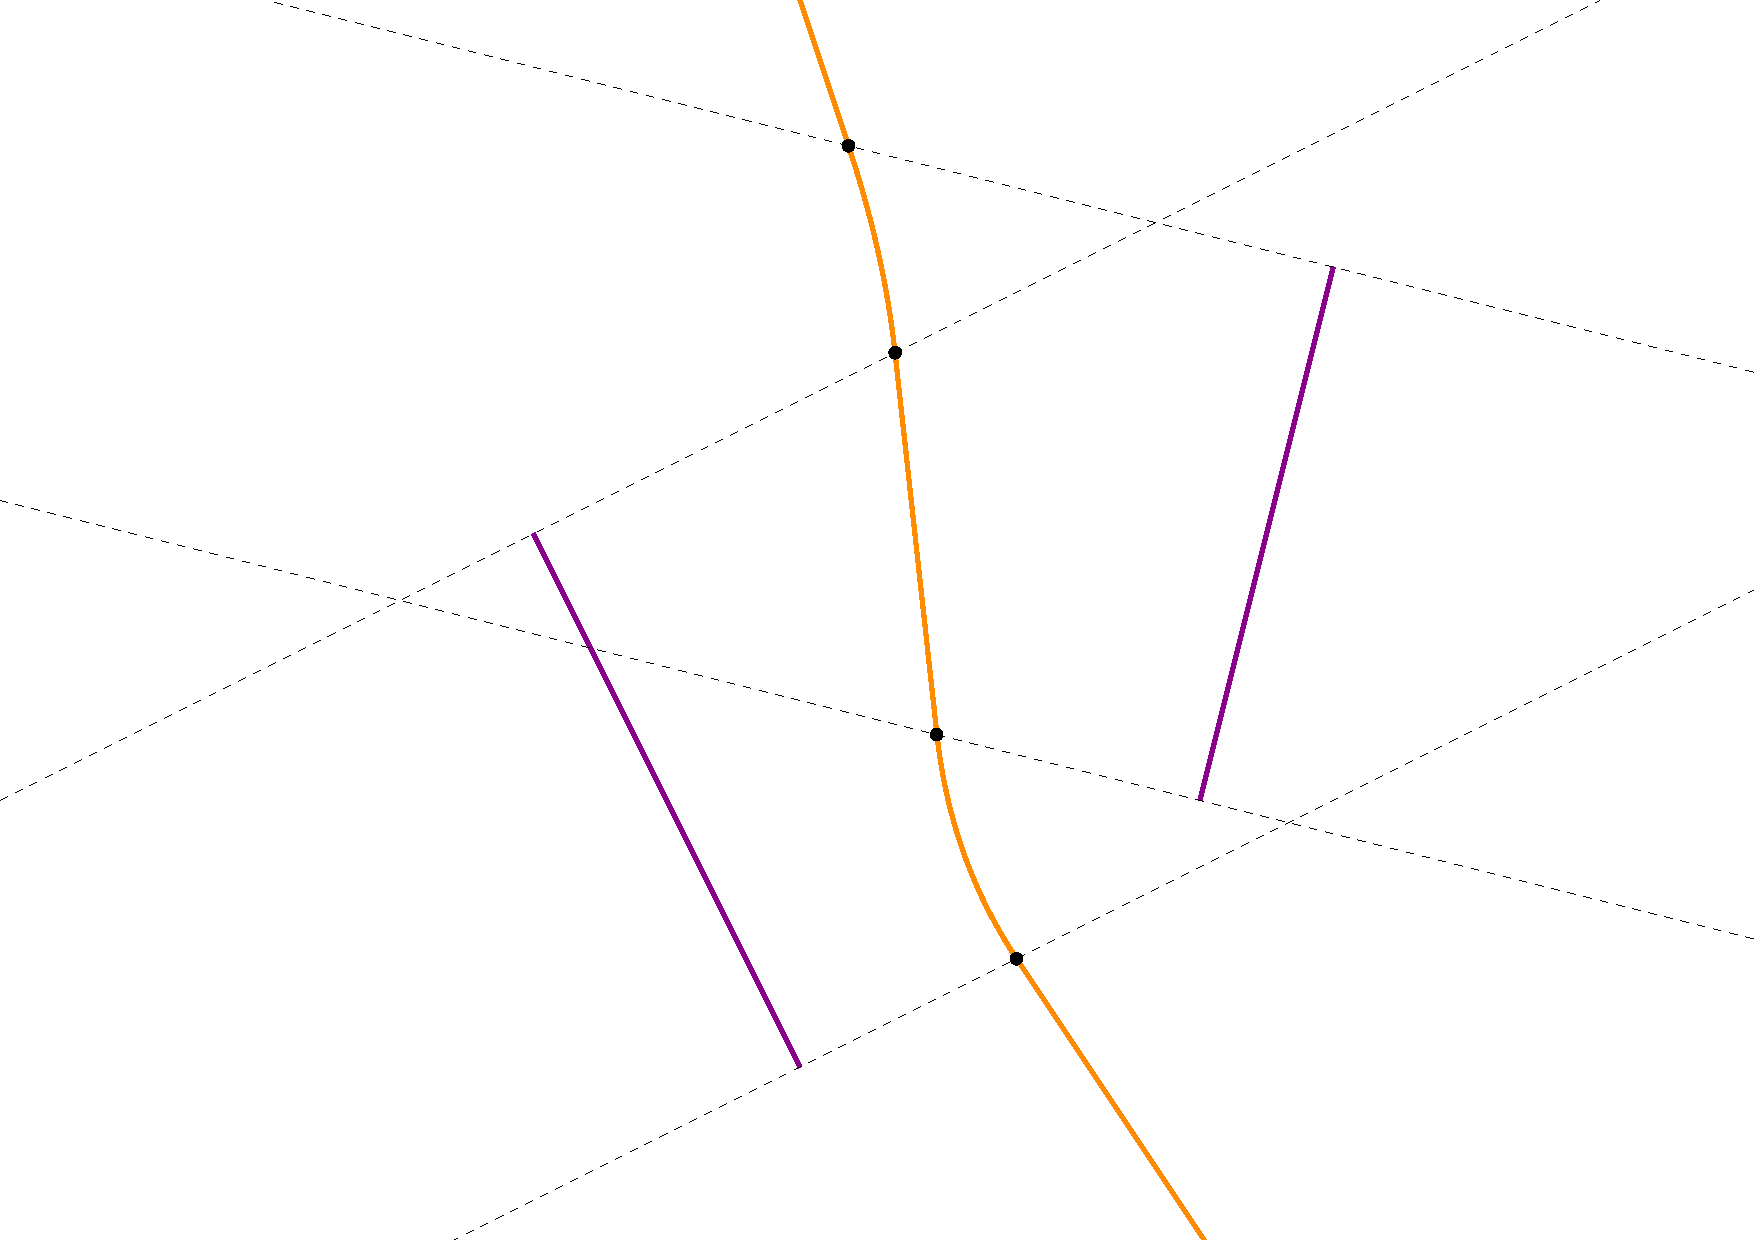
\includegraphics[width=0.8\textwidth]{areas_of_influence}}
    \caption{Different parts of the bisector\label{fig:areas_of_influence}}
	\end{figure}
	Notice how the parts of the bisector are delimited by the lines orthogonal to the segments at their endpoints. For a single segment, these two lines divide the plane in three parts: the points closest to the source of the segment, the points closest to the inner part of the segment, the points closest to the target of the segment.\ppar
	The model of the concept \cod{EnvelopeTraits_3} that was developed is  \cod{L2_segment_voronoi_traits_2} and is parametrised by an Arrangements class from which it inherits, similarly to how the already available model \cod{Env_sphere_traits_3} for envelopes of spheres does; again similarly, the Arrangements class used is \cod{Arr_conic_traits2}.\par
	This Arrangements class defines the geometry of the edges of the diagram, as well as methods for computation of intersections and predicates.
	
	\subsection{Arrangement traits class \cod{Arr_conic_traits2}}
	This class was chosen because it supports construction and computation using conic curves, needed because of the parabolic arcs in the planar euclidean bisector of two segments; such arcs are present in the part of the bisector that is closest to one of the segments' inner part and to one of the other segment's endpoints (see figure \ref{fig:areas_of_influence}).\par
	The curves need to be closed conic arcs lying on a supporting conic curve defined by the equation:
	\[
		rx^{2} + sy^{2} + txy + ux + vy + w = 0 
	\]
	According to the specification (available on the \href{https://doc.cgal.org/latest/Arrangement_on_surface_2/classCGAL_1_1Arr__conic__traits__2.html}{CGAL documentation}), the coefficients (\(r, s, t, u ,v, w\)) need to be all rational numbers. This is because by enforcing this, all intersections between such conic arcs are guaranteed to be algebraic numbers of degree at most 4, and the traits class is optimised for operations with these numbers.\par
	If the supporting conic is not a closed curve such as a circle or an ellipse, and in our case it never is (because it's either a parabola or a line for the straight parts of the bisector), then two endpoints have to be provided. This poses a problem with the unbounded rays (the first and last parts of the bisector, again see figure \ref{fig:areas_of_influence}), because they only have one endpoint.\par
	To obviate this, the rays were cut off at an arbitrary distance: imagine this as if the distance surfaces were not unbounded, but were all limited inside the same large square region. Because of this, the traits class \cod{L2_segment_voronoi_traits_2} also constructs a projected boundary for all surfaces (the same large square boundary for all segments).\par
	Another problem arises when constructing the parts of the bisector that lie on the line that is the bisector of the supporting lines of two segments (the middle part in \ref{fig:areas_of_influence}): all segments are read from the input as rational segments, and have therefore all supporting lines with rational coordinates; this, however, does not prevent the bisector of two such supporting lines to have algebraic coefficients, as can be see in figure \ref{fig:algebraic_line} below. To solve this problem, some approximation was necessary.
	\begin{figure}[h!]
    \centering
    \fbox{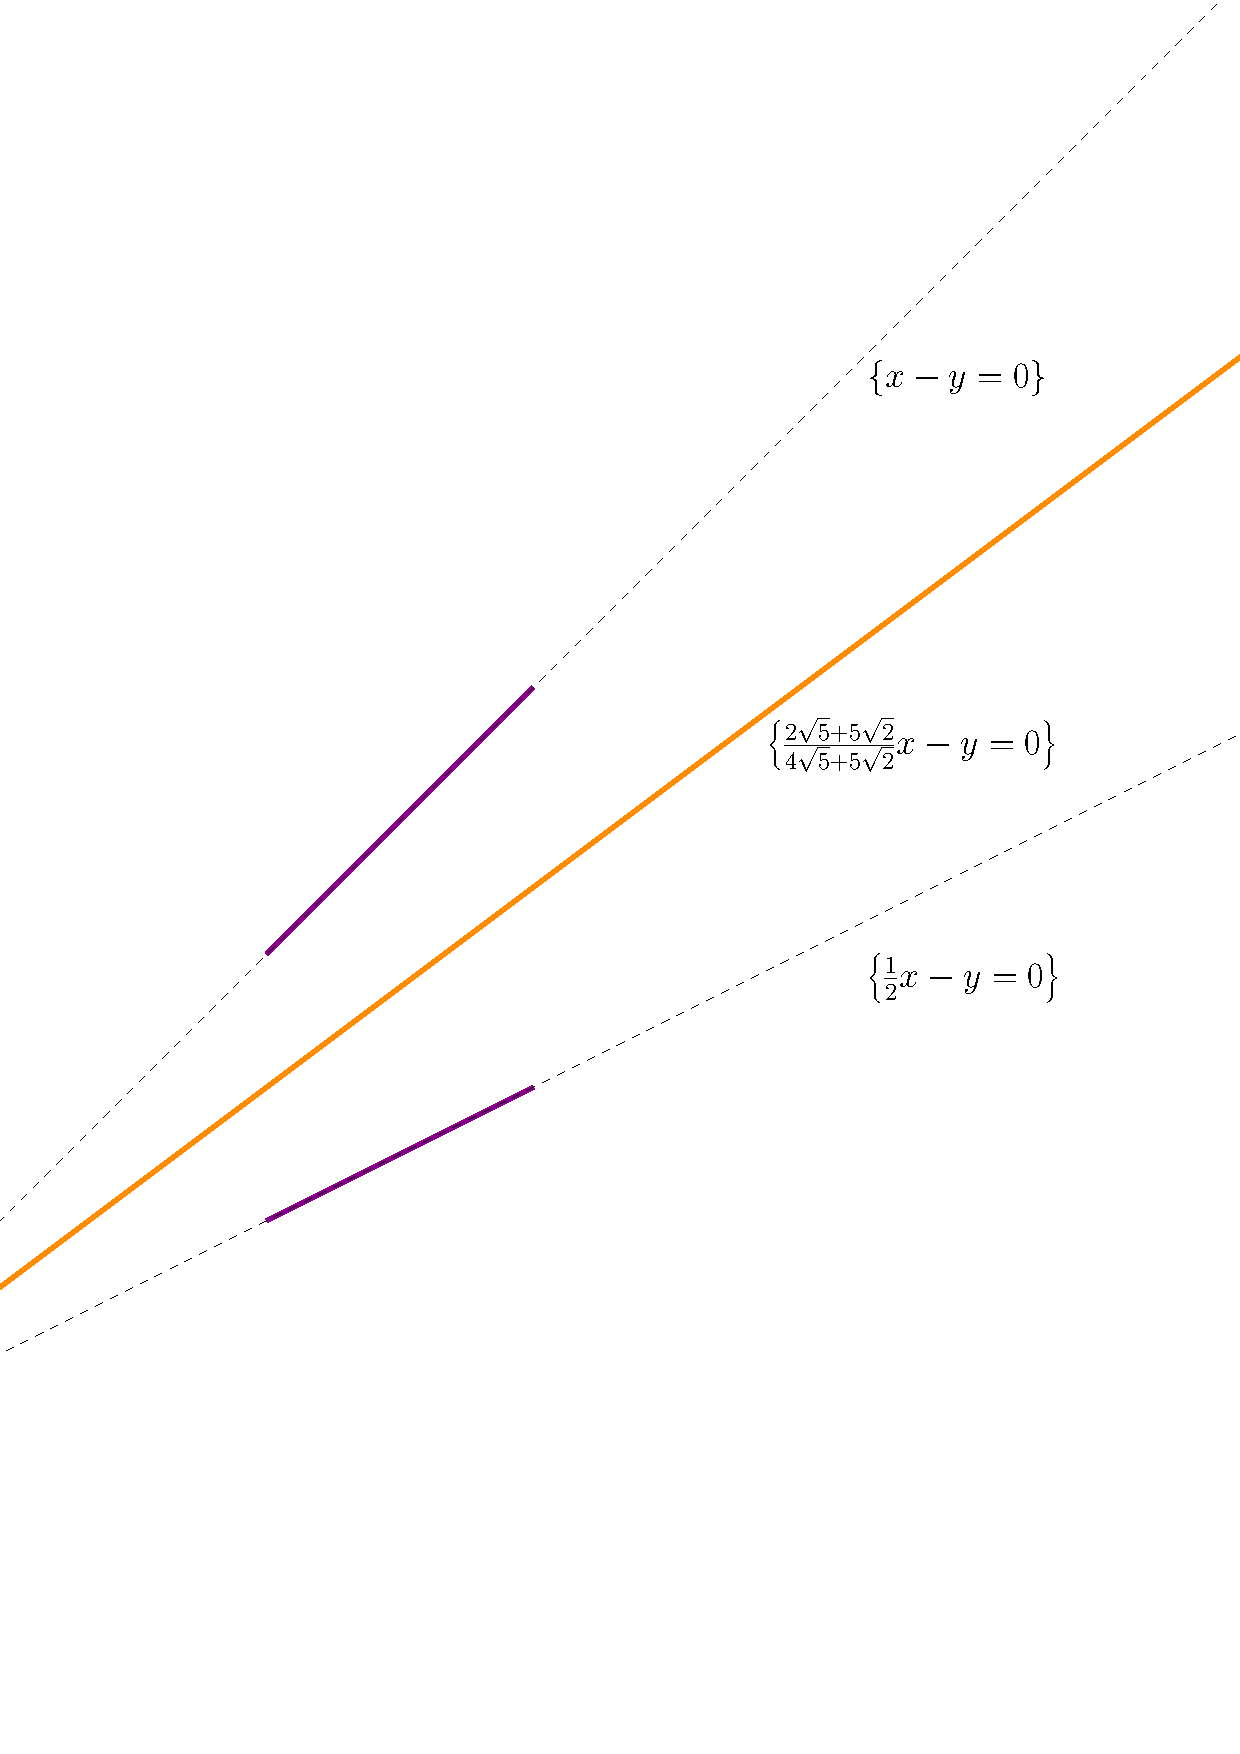
\includegraphics[clip, trim=0 8cm 0 4cm, width=0.6\textwidth]{algebraic_line}}
    \caption{Two segments, their supporting lines and the bisector with algebraic coefficients \label{fig:algebraic_line}}
	\end{figure}
	

	\subsection{\cod{Parabola} class}
	A \cod{Parabola} class was implemented to support construction of parabolas, computation of intersection with lines, construction of arcs on the parabolas and construction of tangent lines at given points on the parabola. Other predicates such as \cod{has_on} were also implemented.\par
	The only constructor for a \cod{Parabola} object takes a focus point and a directrix line. When this class is used in the Ipelet, the directrix and the focus are given as the endpoint of one segment and the supporting line of the other segment accordingly (see figure \ref{fig:parabola}, parabola in green).
	\begin{figure}[h]
    \centering
    \framebox{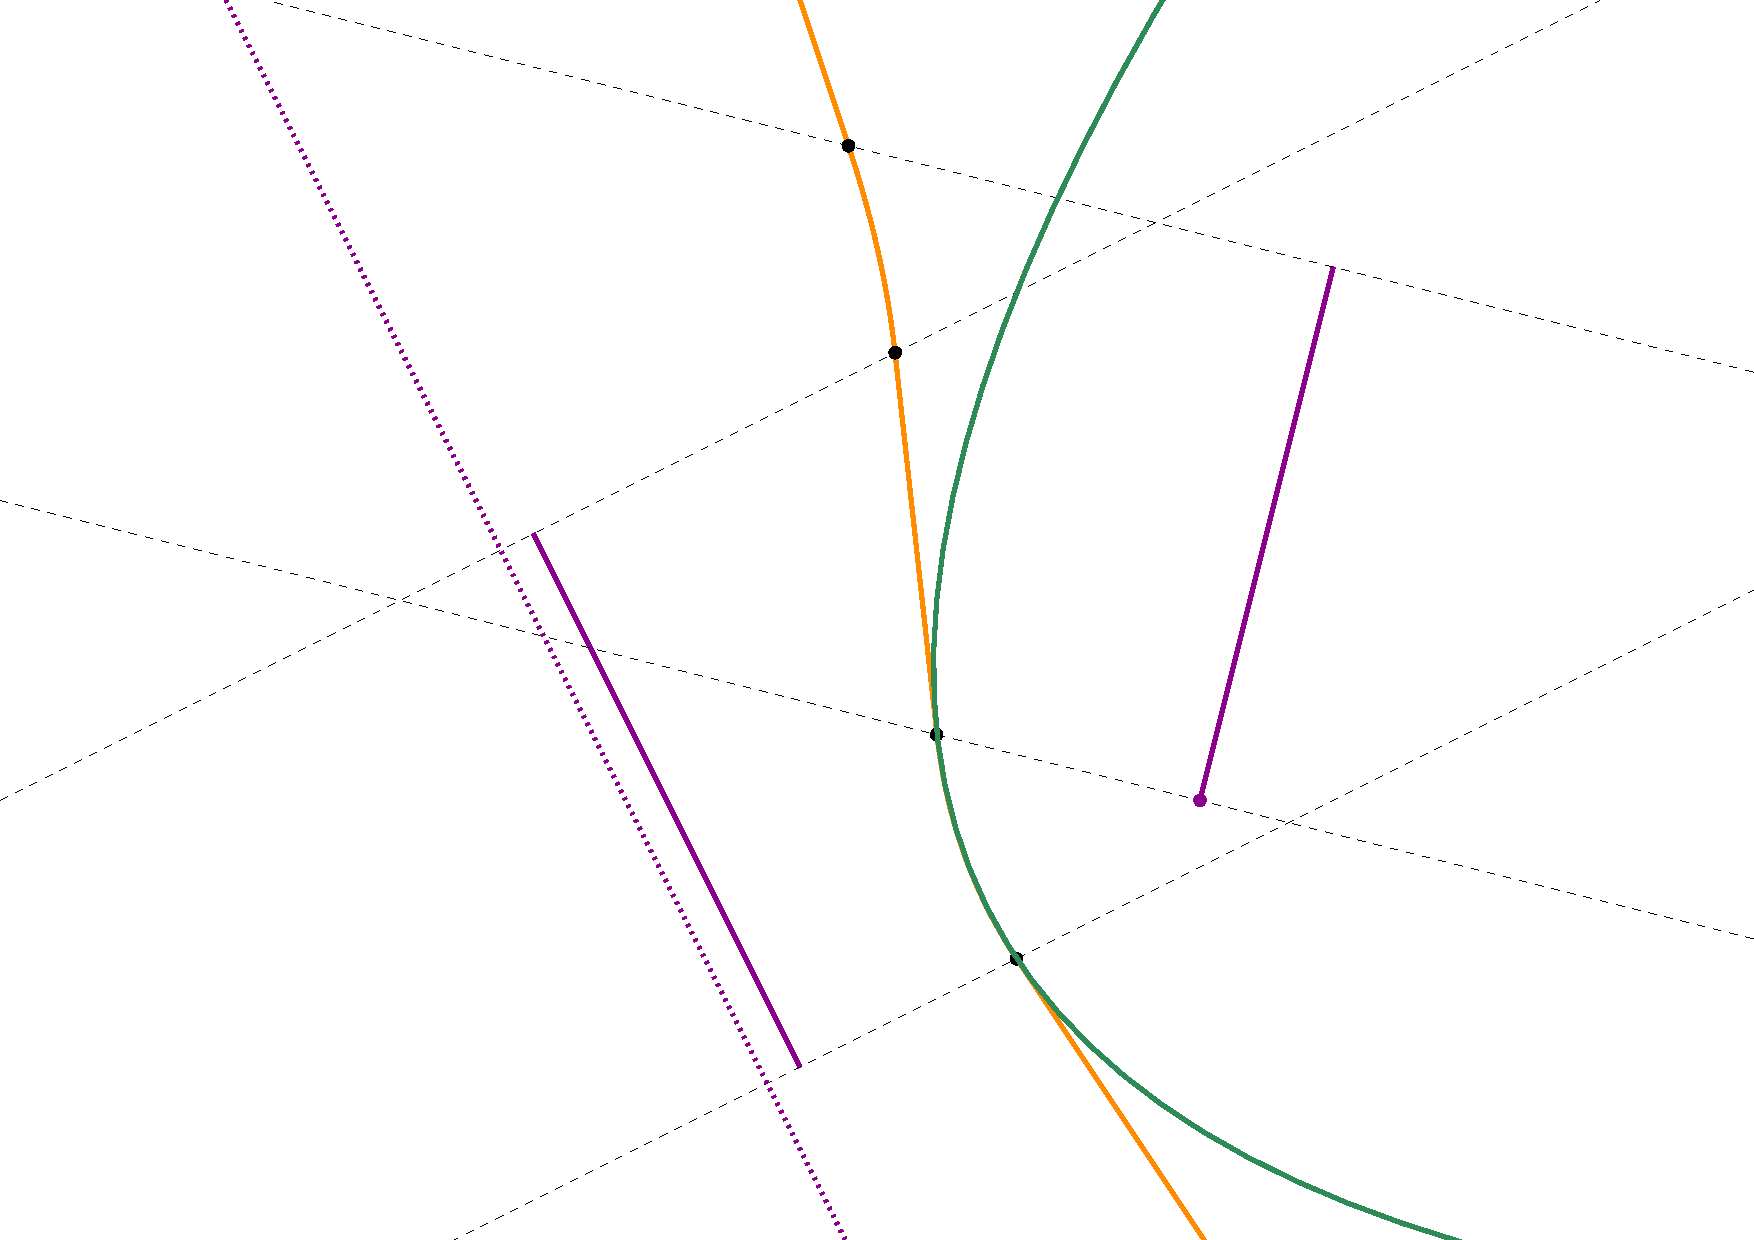
\includegraphics[width=0.8\textwidth]{parabola}}
    \caption{A parabola defined by a supporting line (dotted) and the highlighted endpoint \label{fig:parabola}}
	\end{figure}
	
	
	%____________________________________________________________

	\section{Bisector computation}
	The main part of the project was to implement the functor \cod{Construct_projected_intersections_2} which, as the name suggests, must construct all parts of the \(xy\)-projection of the intersection of two given surfaces. As said before, for FSVD this consists of constructing the bisector of two segments.\par
	The approach used is to first find the unbounded rays and their endpoints.\par
	Then, iteratively construct the rest of the bisector, the internal parts, starting from one ray's endpoint until the other ray's endpoint.
	This is true for the case in which the segments are disjoint; if the segments are intersecting, then there are four unbounded rays, and the bisector is constructed in two iterations, creating two bisectors that "touch" at the intersection of the two segments.\ppar
	
	For both segments, the lines orthogonal to each endpoint are kept saved for the whole computation, since they determine all separations between the bisector parts. In the code, these lines are called \cod{Delimiter_lines}.
	
	\subsection{Unbounded rays}
	\begin{figure}[h]
	\begin{subfigure}[b]{0.3\textwidth}
		\fbox{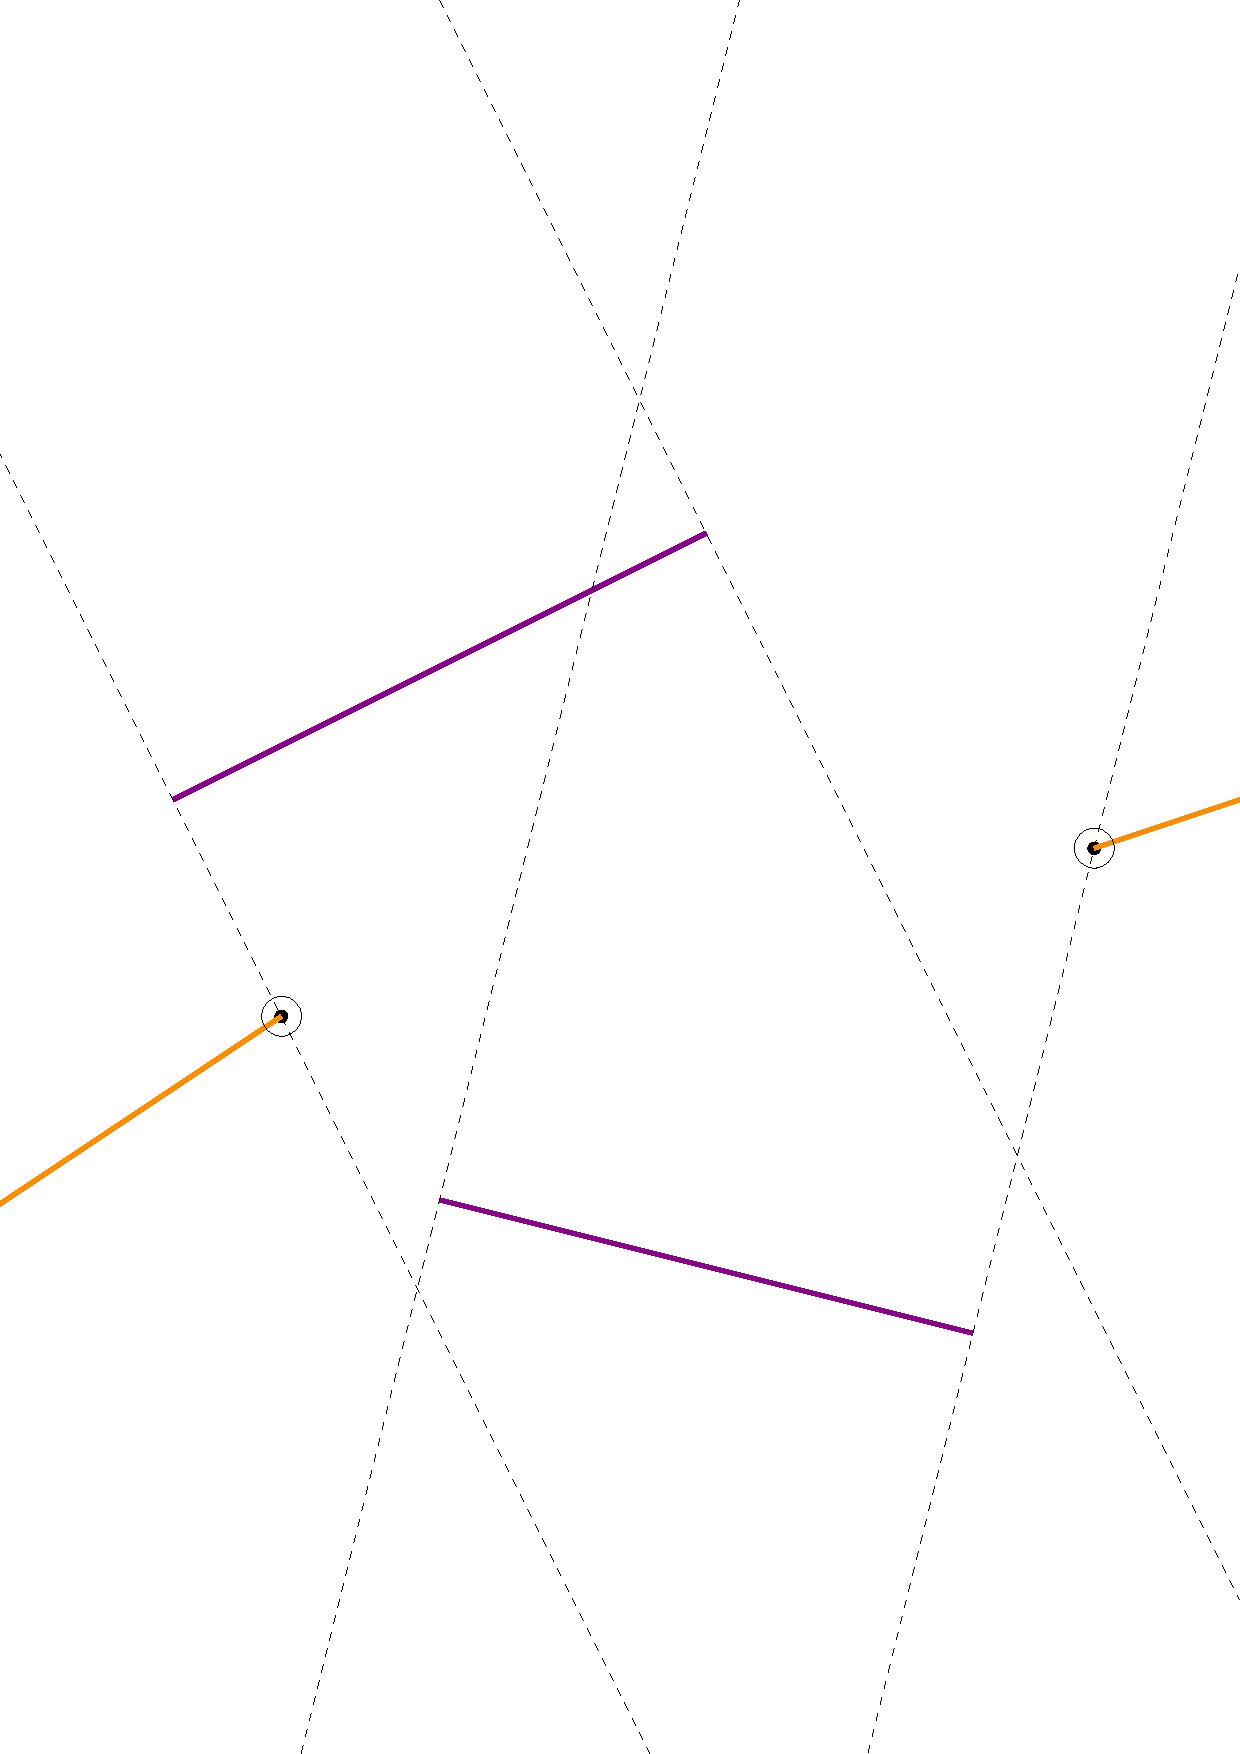
\includegraphics[width=\textwidth]{two_unbounded_rays}}
    	\caption{Disjoint \label{fig:two_unbounded_rays}}
	\end{subfigure}
	\qquad
	\begin{subfigure}[b]{0.3\textwidth}
		\fbox{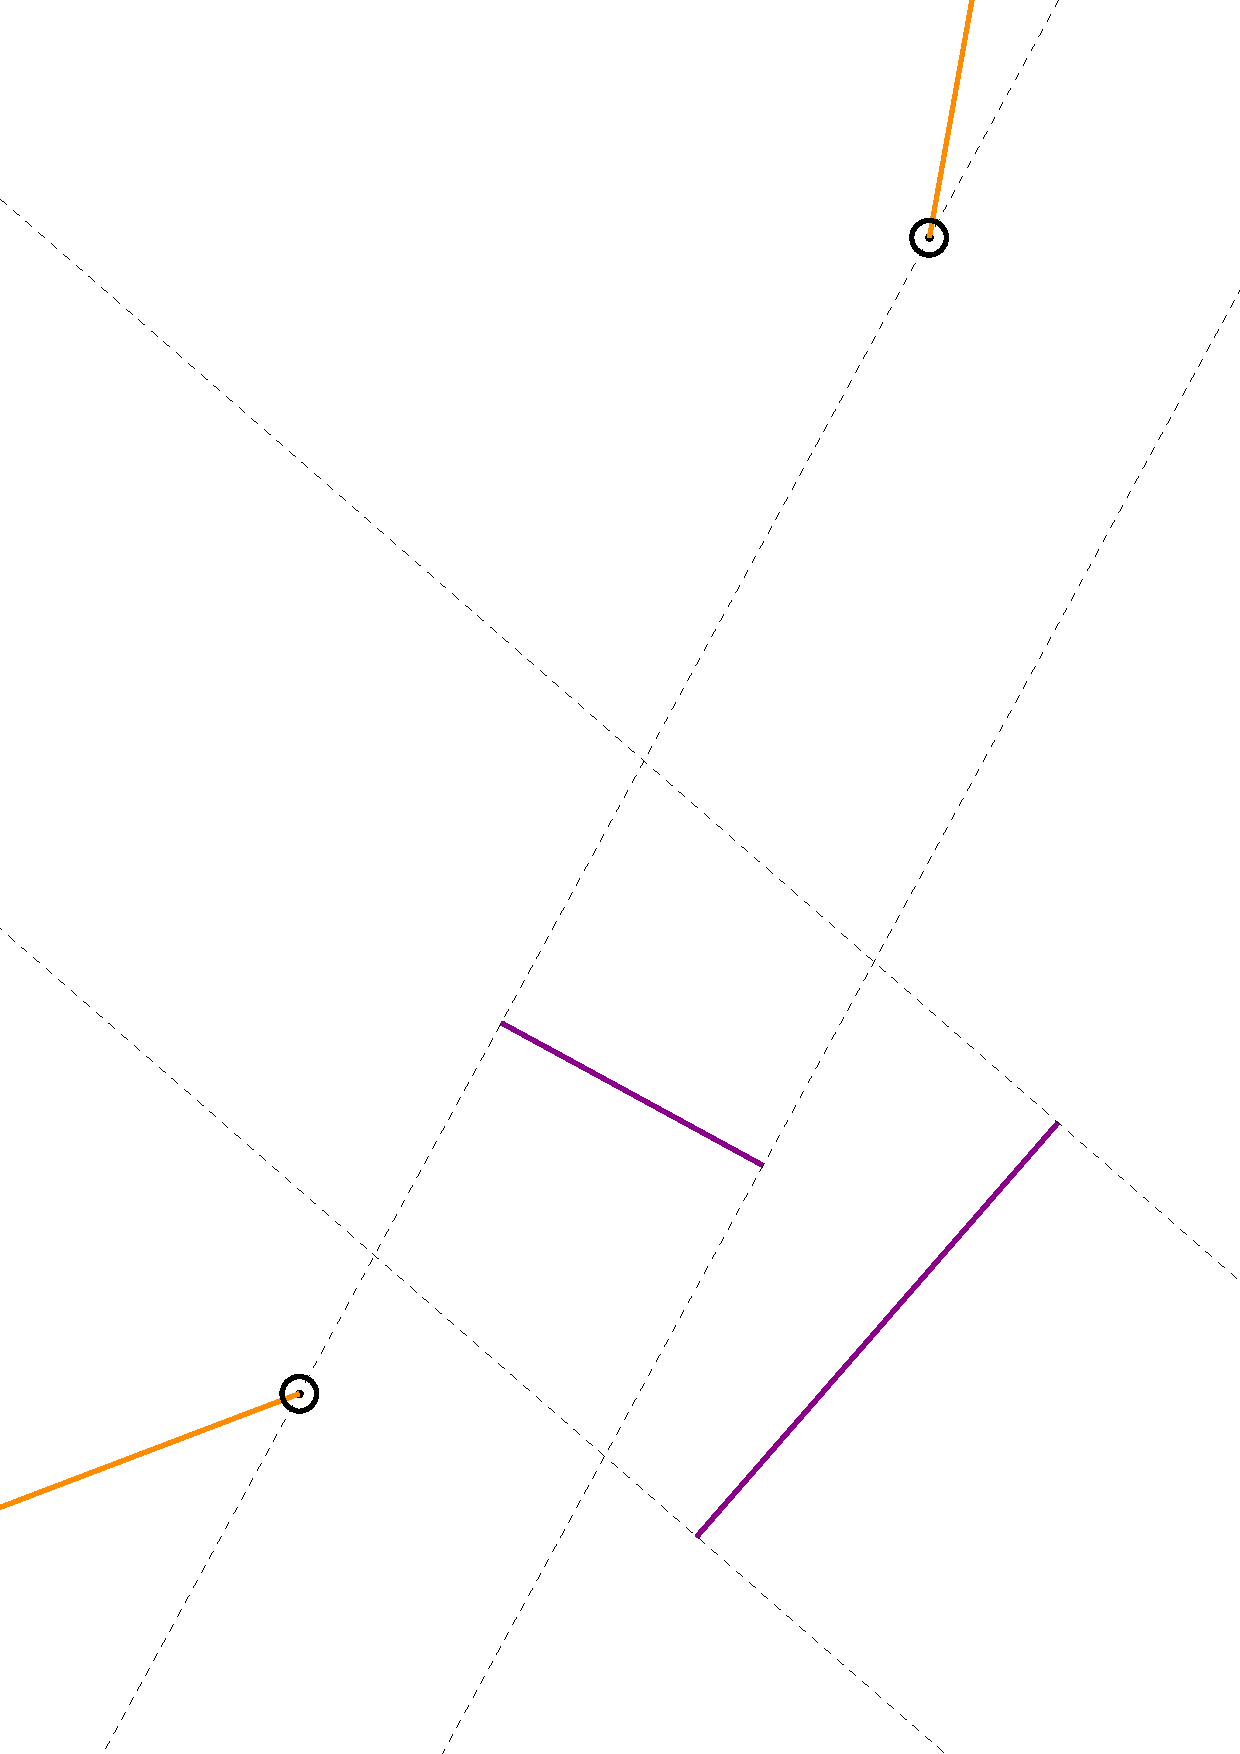
\includegraphics[width=\textwidth]{two_unbounded_rays_2}}
    	\caption{Disjoint 2 \label{fig:two_unbounded_rays_2}}
	\end{subfigure}
	\qquad
	\begin{subfigure}[b]{0.3\textwidth}
		\fbox{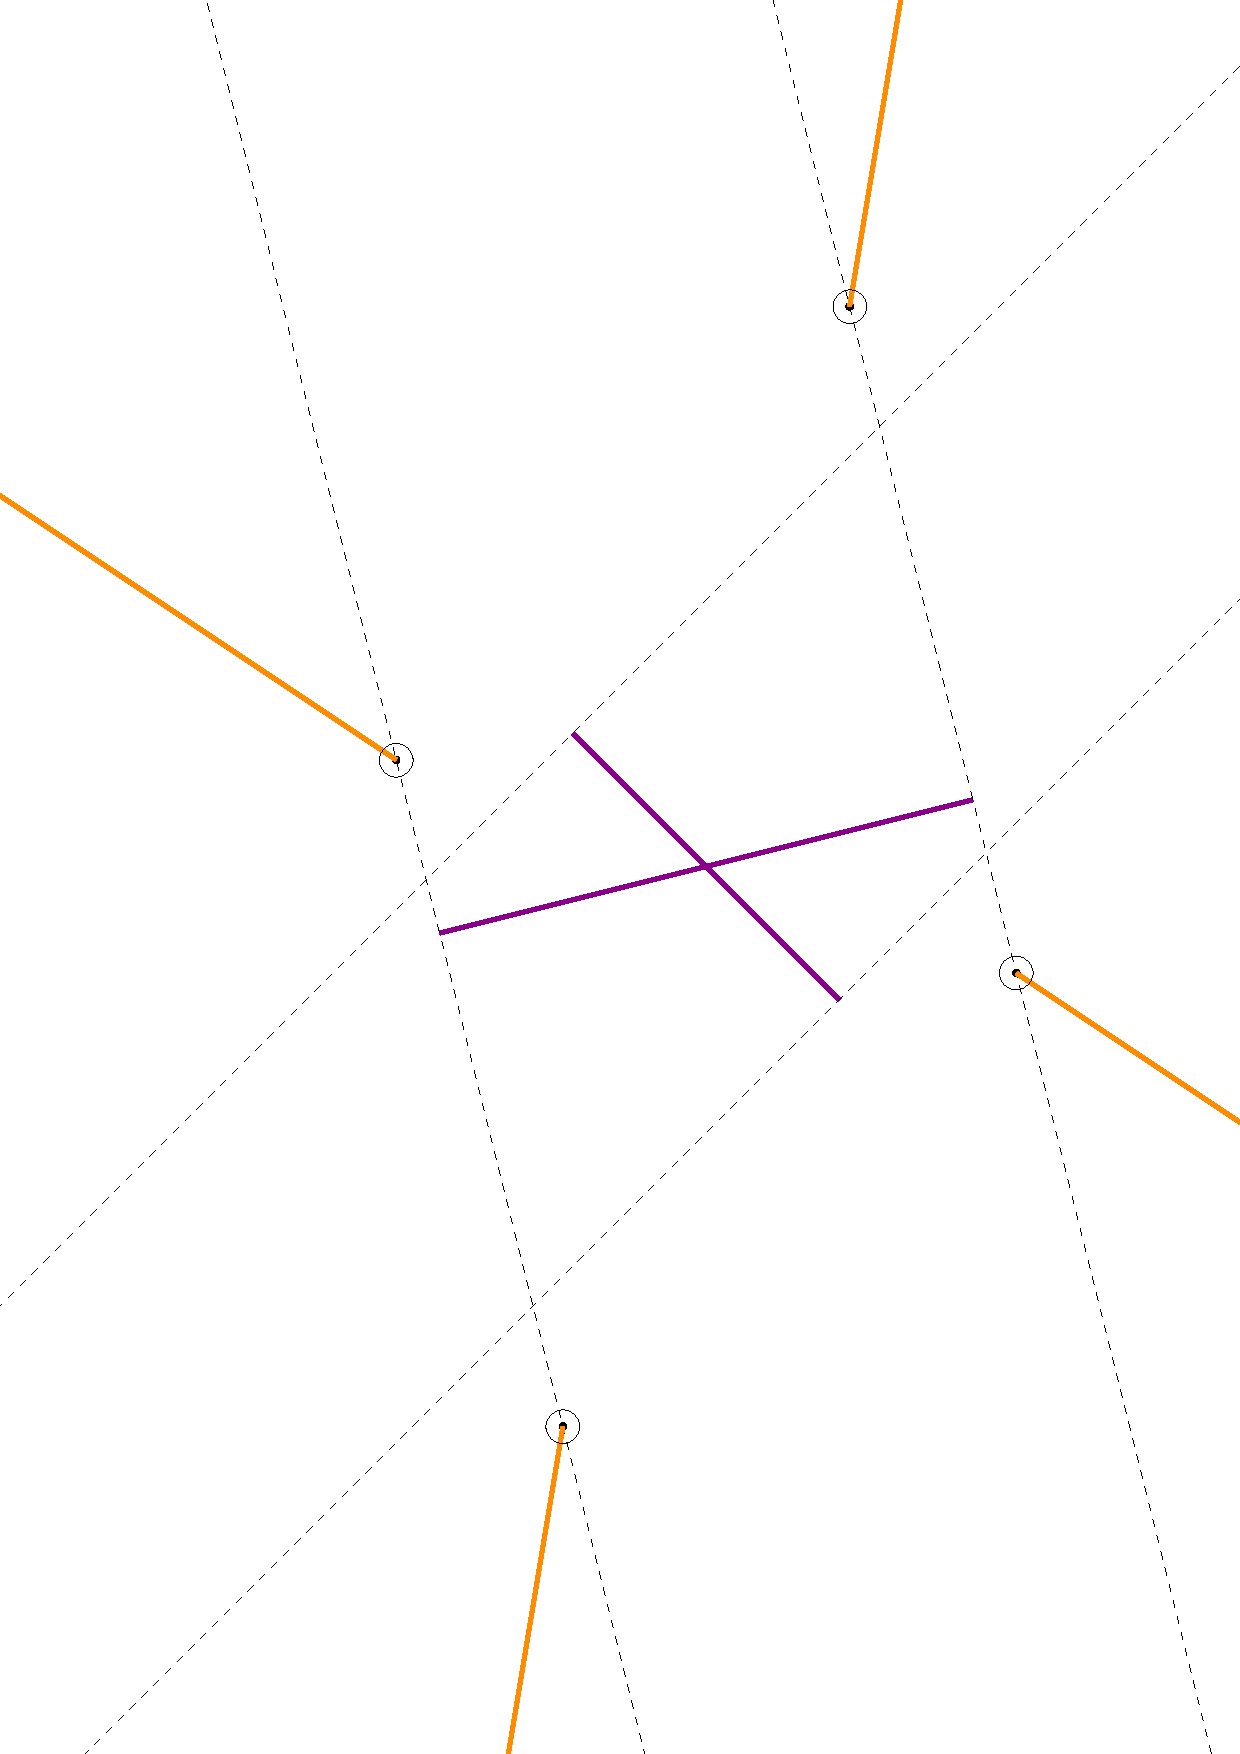
\includegraphics[width=\textwidth]{four_unbounded_rays}}
    	\caption{Intersecting \label{fig:four_unbounded_rays}}
	\end{subfigure}
	\caption{The unbounded rays of the bisector in two cases (in orange)\label{fig:unbounded_rays}}
	\end{figure}
	
	To find the unbounded rays we have to find the bisector of all pairs of endpoints of the two segments that are extremal in the set of the four endpoints of the segments. That is, we find the convex hull of the set of endpoints of the segments, then we construct a polygon with these points. Walking through the edges of this polygon, if the edge is not one of the two segments, trace the orthogonal line through the midpoint of this edge (which is the bisector of the endpoints of the edge) directed towards the outside of the polyogn.\par
	To find the endpoints of a ray, take the farthest intersection of the line (in the direction of the line) with the four \cod{Delimiter_lines}.
	
	\subsection{Internal parts}
	To find the internal parts we implemented the function \cod{construct_bisector_from_point_to_point}; it takes the two segments, a start and an end point (they are the endpoints of two rays).\par
	The computation is iterative, and keeps as status a current point (\cod{curr_pt}) and a current direction (\cod{curr_direction}); it stops when \cod{curr_pt} is the same as the end point.
	At each loop, the algorithm has to decide what kind of segment the next internal part of the bisector is (as an \cod{enum Bisector_type}):
	\begin{itemize}[label=\(\triangleright\)]\setlength{\itemsep}{-2pt}
	\item a parabolic arc \hfill(\cod{PARABOLIC_ARC})
	\item a segment part of the bisector of the two supporting lines \hfill(\cod{SUPP_LINE_BISECTOR})
	\item a segment part of the bisector of two endpoints \hfill(\cod{ENDPOINT_BISECTOR})
	\end{itemize}
	To do this, based on the \cod{curr_direction} and starting from \cod{curr_point}, shoot a straight line until the next intersection with the \cod{Delimiter_lines} is found (see figure \ref{fig:iteration_shoot}). Then take the midpoint between \cod{curr_pt} and the next intersection found (called \cod{approximate_next_intersection} in the program). Determine where this midpoint is, based on the orientation of the \cod{Delimiter_lines} (they always have their segment on the negative side) and on the predicates \cod{has_on_positive_side} and \cod{has_on_negative_side}.
	
	\begin{figure}[h]
    \centering
    \framebox{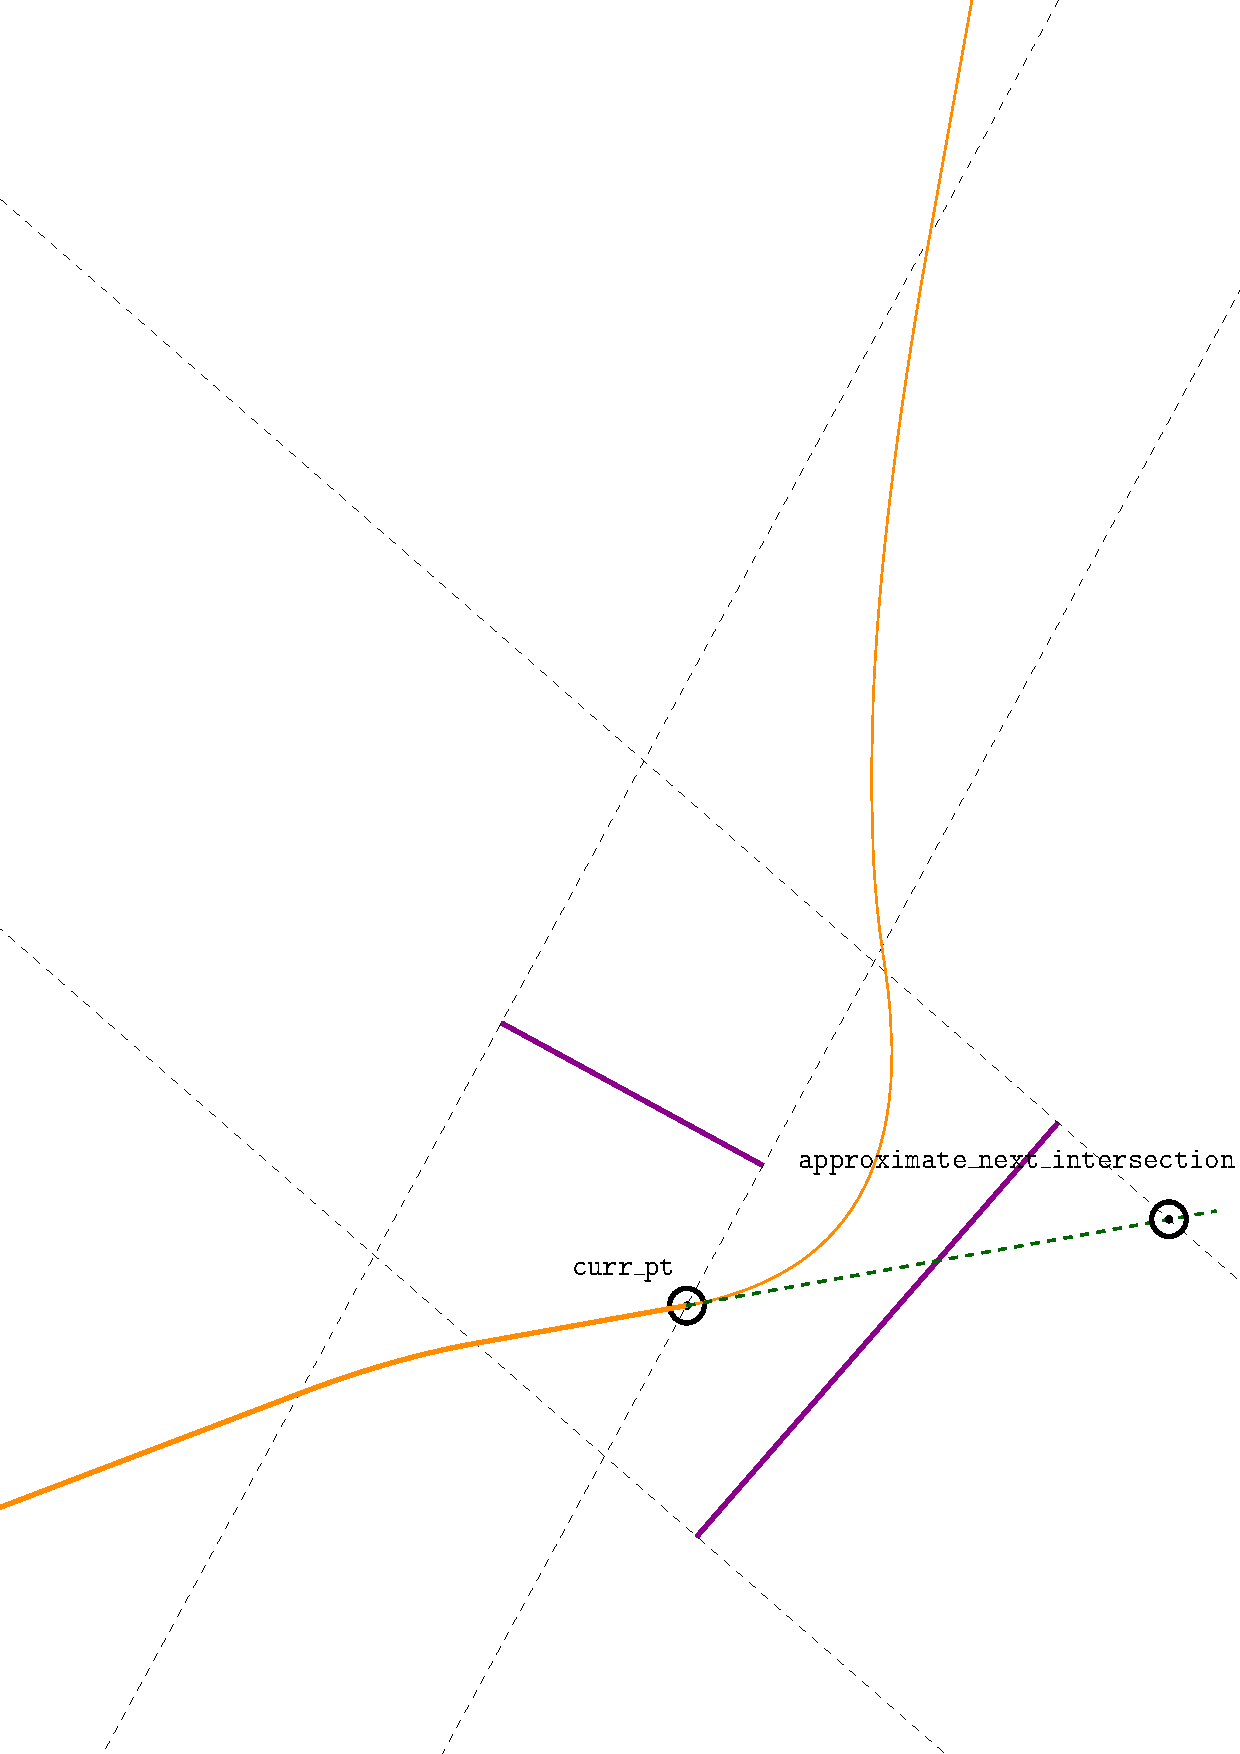
\includegraphics[clip, trim=2cm 2cm 0 12cm, width=0.8\textwidth]{iteration_shoot}}
    \caption{Step in the iteration. Previous parts in bold orange, future parts in thin. \label{fig:iteration_shoot}}
	\end{figure}
	
	Once determined in which case of the three (\cod{PARABOLIC_ARC}, \cod{SUPP_LINE_BISECTOR} or \cod{ENDPOINT_BISECTOR}) we are, construct a parabolic arc or a segment, then find the real next intersection with the \cod{Delimiter_lines}, update the \cod{curr_pt} and the \cod{curr_direction}.
	
	\subsection{Disjoint and intersecting segments}
	For this iteration, as said, there are two main cases: either the segments are disjoint, or the segments are intersecting; the case in which the intersection is weak (i.e. one segment just touches the other by an endpoint) was not taken into account.\par
	To distinguish between these two cases, it suffices to check using the provided \cod{CGAL::do_intersect} function. If the segments do not intersect, then there are only two unbounded rays constructed. If they do intersect, there are four unbounded rays.
	\subsubsection{Disjoint segments}
	In this case, there are two rays, so just start from one ray and iterate constructing all internal parts of the bisector until the other ray (the endpoint) is found. In this case there are no real struggles, even when adding the approximation for the algebraic parts as described below.
	\subsubsection{Intersecing segments}
	In this case, there are four rays, therefore the iteration has to be done two times. The bisector can be seen as two bisectors that meet at the intersection of the two segments.\par
	At first, the idea was to just make the two bisectors cross in the middle, but after a first implementation we observed that in this way they were not logically correct. Each bisector started by having one segment on the left side and the other on the right side; after the intersection, however, the two segments were in the opposite sides.\par
	Therefore, it was decided to change the implementation to have the two bisectors touch at the segments intersection and then turn away from each other, maintaining the side on which the segments were for both bisectors (see figure \ref{fig:intersecting_bisectors}).
	\begin{figure}[h]
    \centering
    \framebox{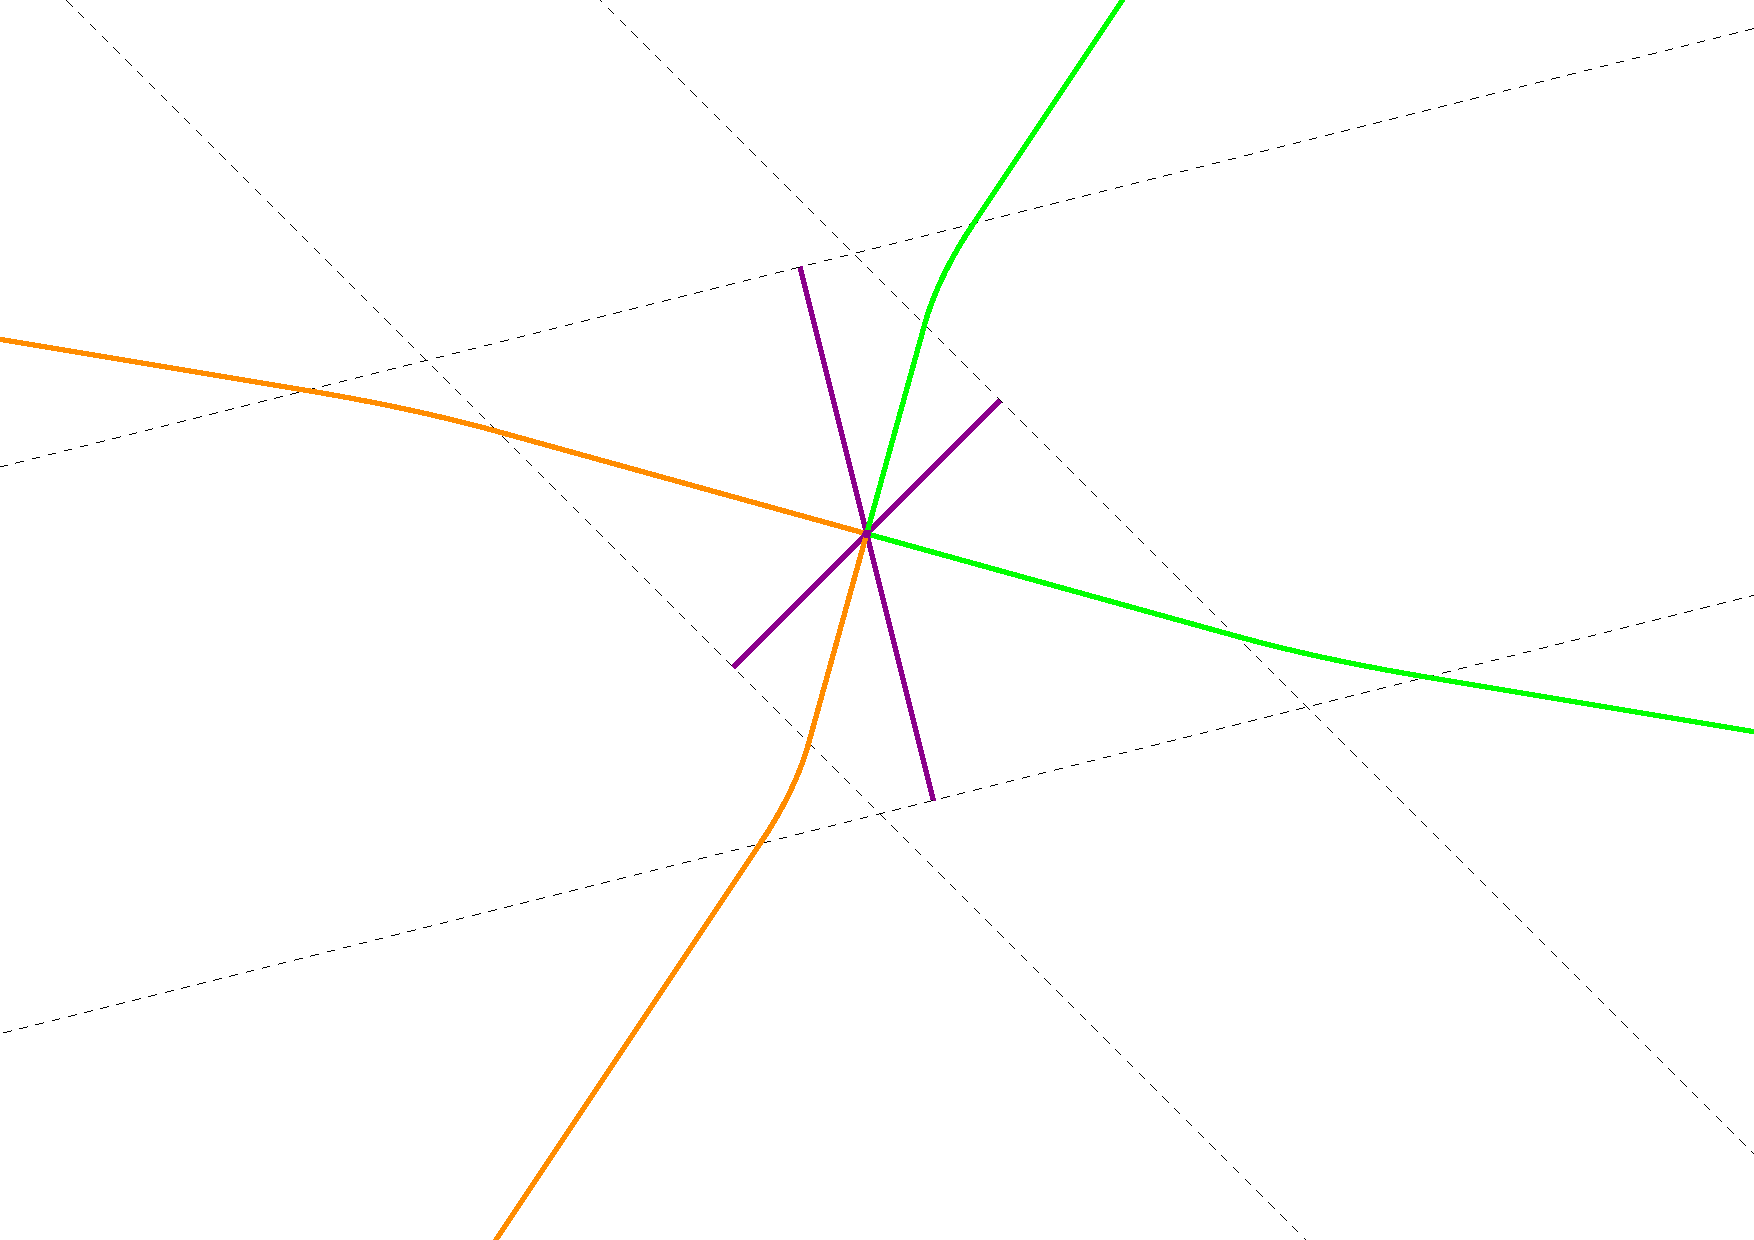
\includegraphics[clip, trim=2cm 2cm 2cm 2cm, width=0.8\textwidth]{intersecting_bisectors}}
    \caption{The two lines (in orange and green) constituting the bisector of two intersecting segments. \label{fig:intersecting_bisectors}}
	\end{figure}
	
	\subsection{Approximation}
	The main problem with the computation of the bisector were the parts that lie on the bisector of the supporting lines of the two segments. This is because even if the two segments lie on lines with rational coefficients, the bisector might potentially have algebraic coefficients, as shown in figure \ref{fig:algebraic_line} previously.\ppar

	As said before, the class \cod{Arr_conic_traits2} allows to construct only \cod{Curve_2} objects that lie on curves that have rational coefficients. An algebraic segment has as supporting curve a line that has algebraic coefficients.\par
	To save it, it needs to be slightly approximated. To do it, the two endpoints of the algebraic segment are moved sligtly so that the supporting line  is either translated or rotated, but it still intersects the previous and the next parts of the bisector (in the general case they are parabolic arcs). This is done in such a way that the approximated supporting line has rational coefficients.\par
	To know in which direction to translate/rotate the segment, it suffices to look at the direction of the segment and the orientation of the previous arc and the next arc.\par
	Fortunately then, the \cod{Arr_conic_traits2} class provides a constructor for a \cod{Curve_2} object that takes:
	\begin{itemize}[label=\(\triangleright\)]\setlength{\itemsep}{-2pt}
		\item the coefficients of the supporting conic of the curve (so the ones of the approximated line)
	\item the orientation of the curve (collinear, since it's a segment)
	\item the approximations of two endpoints of the curve (the endpoints of the original algebraic segment are given, which are exact)
	\item the coefficients of the supporting conic of the previous arc
	\item the coefficients of the supporting conic of the next arc
	\end{itemize}
	
	\subsection{Drawing}
	The \cod{CGAL_Ipelets} package has many methods to draw geometric figures; it does not support, however, the drawing of conic arcs. Because of this, the arcs are converted to sets of very small segments. This is done just at the end, when the diagram is already ready to be drawn: the Ipelet asks user input for a precision value for the conversion of the arcs to sets of small segments. Lower values take a really long time.
	
	%____________________________________________________________
	\section{Results and future work}
	
	\subsection{Ipelet functionality}
	The Ipelet correctly computes the bisector of two segments in general cases.\par
	For three segments, the FSVD and SVD diagrams are usually correct. For intersecting segments, the Ipelet works less well. By checking the console output it is possible to see all checks performed, and everything seems to be working correctly; the graphical output is, however, wrong.\ppar
	To see the output, simply run the Ipe app from command line; the executable is found at: \cod{/Applications/Ipe.app/Contents/MacOS/ipe}.
	
	\subsection{Known limitations}
	\begin{enumerate}
	\item The Ipelet does not work if there is any pair of segments such that there are three points that are collinear: this is because the computation of the convex hull to find the unbounded rays would leave the middle collinear point out of the hull, but it should be included for the idea used.
	\item If any two segments are touching, the Ipelet also does not work correctly, because one part of the bisector is not included (the one shooting orthogonally to the segment at the contact point with the other segment).
	\item The ipelet does not work if there are degenerate segments (points) in the input set. If all segments are degenerate, though, it works fine, since the problem degenerates to a Voronoi diagram for points.
	\end{enumerate}
	
	\subsection{Issues}
	\begin{enumerate}
	\setcounter{enumi}{3}
	\item For two segments that are \emph{horizontal}, parallel and of the same length, the Ipelet crashes because of an error in the \cod{Envelopes} package, a violated precondition. Before the crash there is also a warning: \cod{"Explanation: Found two vertices with the same geometric point."}.
	\item The Ipelet also draws the fake boundary of the diagram (the one used to bound the unbounded rays). It is only visible by zooming out to the maximum and by panning the canvas a bit towards the sides (in any direction). This is a minor issue.
	\end{enumerate}
	
	\subsection{Alternatives and possible solutions}
	First of there are some solutions for the listed limitations and problems (from 1 to 4):
	\begin{enumerate}
	\item Two disjoint segments with three endpoints collinear: this is simply a problem with the computation of the convex hull of the four endpoints. The middle collinear point is left out, therefore one of the unbounded rays is constructed wrongly. To solve this, there are two ways that were only though of but not implemented:
	\begin{itemize}[label=\(\triangleright\)]\setlength{\itemsep}{-2pt}
		\item create/modify a convex hull algorithm for the set of four points that keeps the middle of three collinear points if it would be on the edge of the hull. With this, the algorithm should work correctly.
		\item create a special case (at the beginning of the method, where other special cases are handled) to handle this. This case would only need to get the unbounded rays correctly, and the internal parts could still be computed using the iterative method (by calling the function \cod{construct_bisector_from_point_to_point}).
	\end{itemize}
	\item Touching segments: this case should be dealt with as a special case. There was little time to implement this because already the general case had many hidden difficulties and still does not work properly.
	\item Mixed input (segments and points): to implement this, it is sufficient to implement the case at line \cod{1377}, with the comment \cod{//TODO bisector of point and segment}. This case was just ignored because it was easy to do and not really important.
	\item Weird crash for horizontal parallel and same length segments: this case needs to be debugged by looking into the \cod{Envelopes} package.
	\item Drawing of fake boundary: to avoid drawing this boundary one needs to correct the method \cod{on_boundary} at line 230 in the file \cod{bisectors.cpp}. This function simply checks if the edge of the diagram to be drawn is a piece of the drawing itself, and if it returns true the edge is not drawn.\par
	The current implementation was written really fast and fails in a special case, when the diagram contains a single line that starts and ends on the boundary itself.
	\end{enumerate}
	
	\subsubsection{\cod{Arr_linear_segment_traits_2}}
	As said, the \cod{Arr_conic_traits_2} class only supports bouded curves, and the unbounded rays needed therefore to be converted into long segments by introducing an arbitrary boundary for all distance surfaces.\par
	To avoid this, it would be possible to use the more recent class \cod{Arr_linear_segment_traits_2}. This class allows the curves to be any kind of curves of the form:
	\[
		\sum_{i+j \leq n} a_{ij} x^{i}y^{j} = 0
	\]
	This of course includes conic arcs. The coefficients \(a_{ij}\) need to be integer numbers (so also rational, by just multiplying all of them to make them into integers), so the approximation of the algebraic parts of the bisector would still be necessary.\par
	This, however, would allow to use unbounded rays; it is unknown if the current implementation with the fake boundary actually causes problems.\par
	This approach was at first discarded because of the complexity of the \cod{Arr_linear_segment_traits_2} class; it could, however, even be more efficient.
	
	\subsubsection{Own Arrangements class}
	Another possibility would be to implement an own model of \cod{EnvTraits} containing also an implementation of the Arrangements class methods. Doing so, it might be possible to remove the approximation by allowing segments lying on algebraic curves. This could however increase the mathematical complexity of the computation of intersections.
	
\end{document}
